\section{Methods}
Describe the methods used. How it works. It can include algorithms, system descriptions, new language constructs, analyses, etc.
Provide diagrams to help in the discussion. Figure \ref{fig:one-col-figure} and Figure \ref{fig:two-col-figure} shows an example of a one-column figure and a two-column figure. 
\begin{figure}
    \centering
    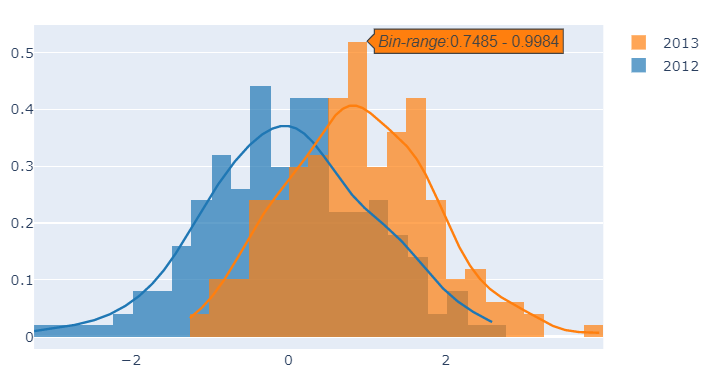
\includegraphics[width=\linewidth]{figures/example_plot.png}
    \caption{One-column figure that explains the steps or framework of your method / model.}
    \label{fig:one-col-figure}
\end{figure}

\begin{figure*}
    \centering
    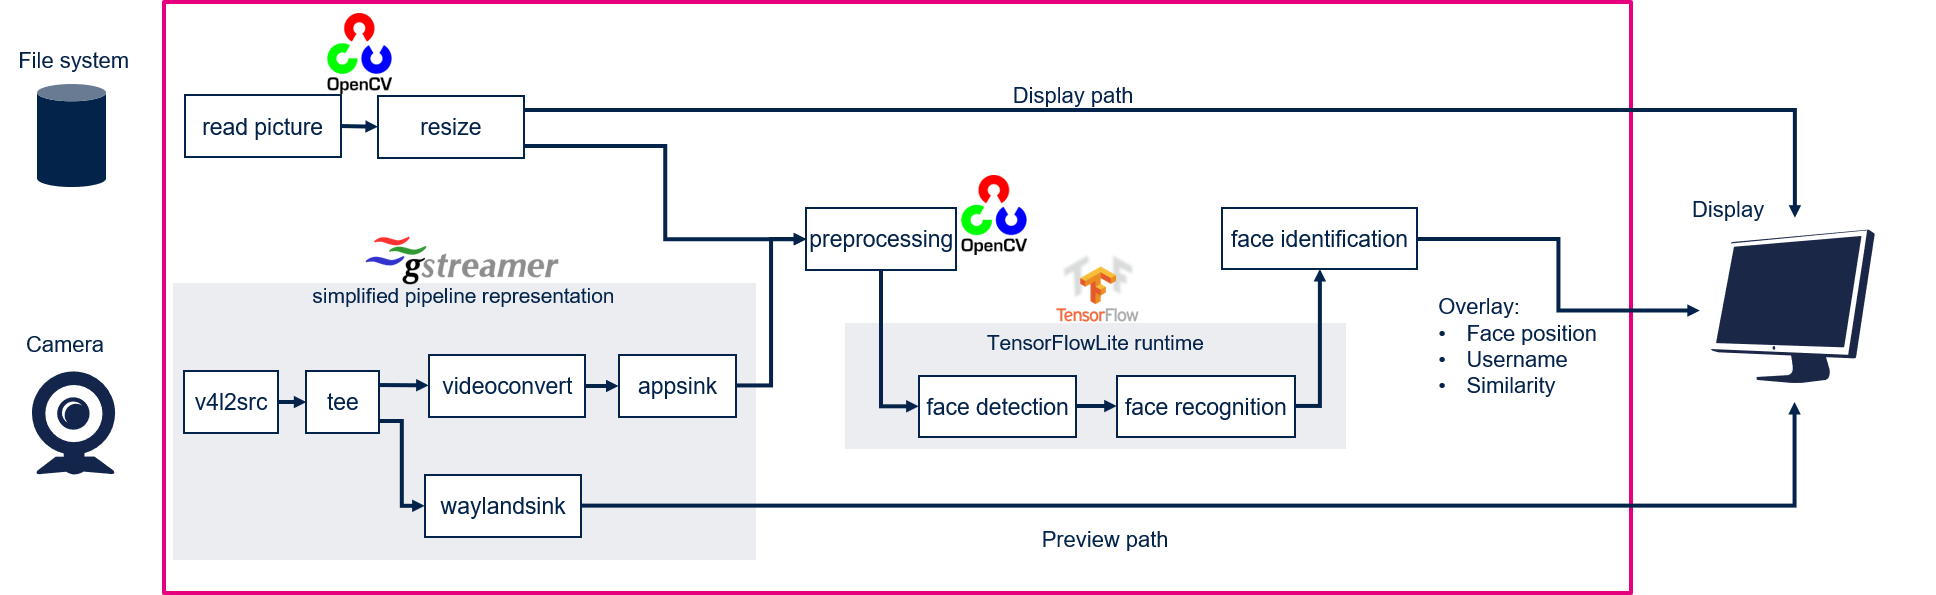
\includegraphics[width=\linewidth]{figures/example_pipeline.png}
    \caption{One-column figure that explains the steps or framework of your method / model.}
    \label{fig:two-col-figure}
\end{figure*}
